% groupplot_no_style.tex -- self-contained standalone figure (no shared style needed)
\documentclass[tikz]{standalone}
\usepackage{pgfplots}
\pgfplotsset{compat=1.18}
\usepgfplotslibrary{groupplots}
\usepackage{siunitx}

\begin{document}
\begin{figure}[h!]
\centering
\resizebox{\linewidth}{!}{
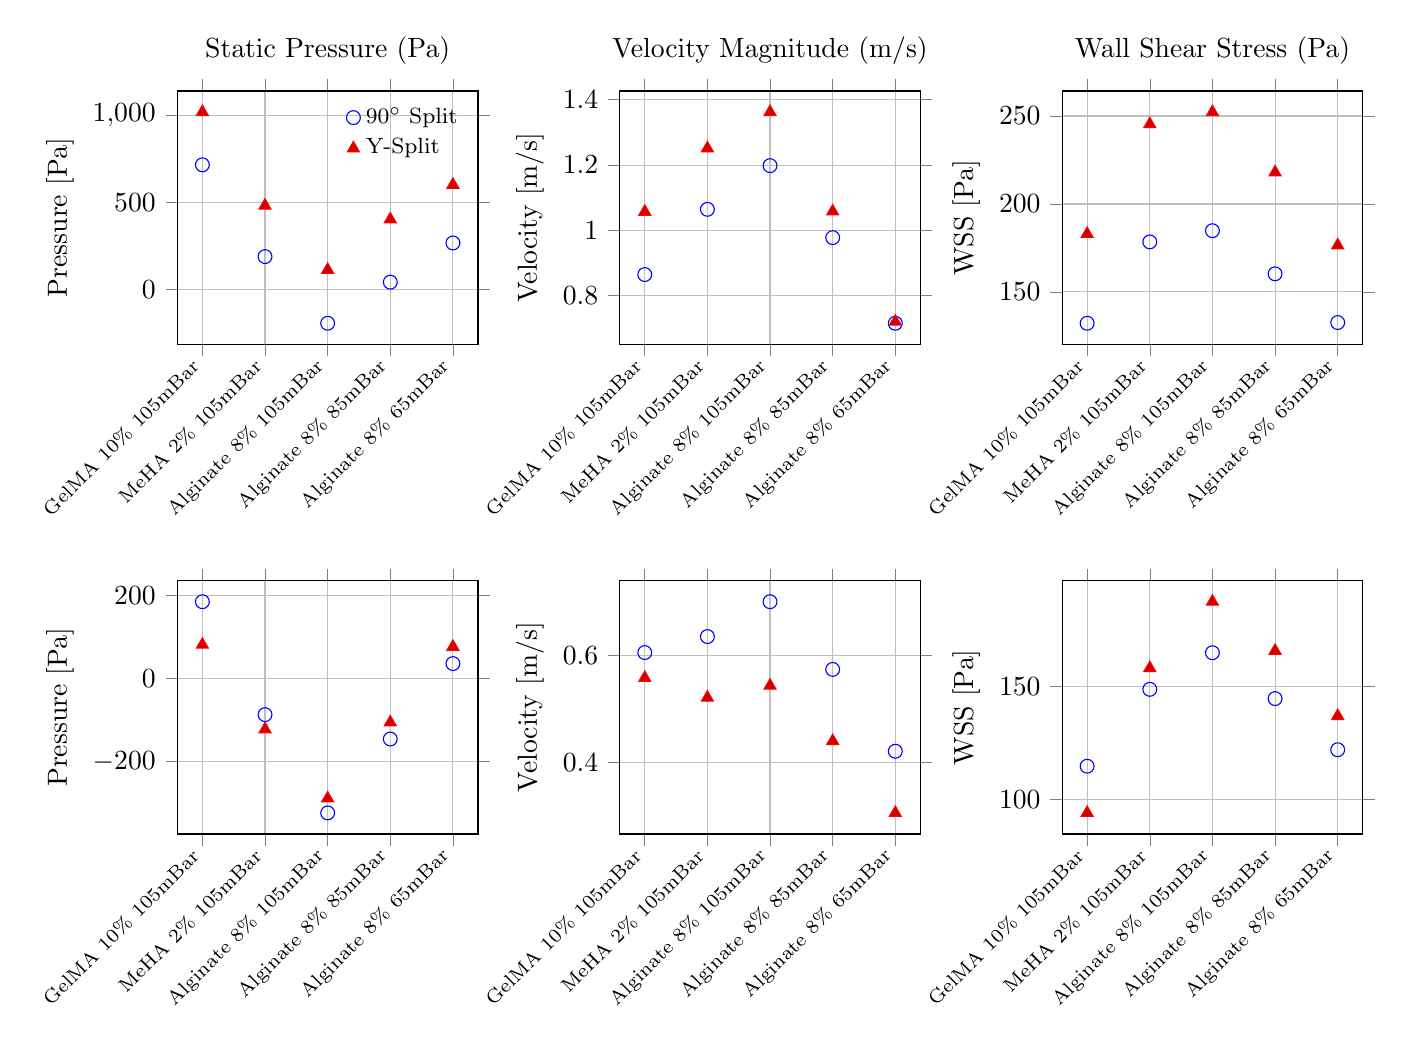
\begin{tikzpicture}
\begin{groupplot}[
  group style={
    group size=3 by 2,
    horizontal sep=18 mm,   % more space between columns
    vertical sep=30mm       % more space between rows
  },
  width=5.4cm, height=4.8cm,
  ymajorgrids, xmajorgrids,
  tick align=outside,
  xtick=data,
  xticklabel style={
    rotate=45,
    anchor=east,
    font=\scriptsize       % smaller labels to reduce clash
  },
  symbolic x coords={
    {GelMA 10\% 105mBar},
    {MeHA 2\% 105mBar},
    {Alginate 8\% 105mBar},
    {Alginate 8\% 85mBar},
    {Alginate 8\% 65mBar}
  },
  legend cell align=left,
  legend style={draw=none, fill=none, font=\footnotesize}
]

% ----------------- Row 1: TWO OUTLETS -----------------

% (1,1) Pressure 2-out
\nextgroupplot[title={Static Pressure (Pa)}, ylabel={Pressure [Pa]}]
\addplot+[only marks, mark=o, mark size=2.5pt] coordinates {
  ({GelMA 10\% 105mBar},  715.06)
  ({MeHA 2\% 105mBar},    188.25)
  ({Alginate 8\% 105mBar},-194.45)
  ({Alginate 8\% 85mBar},  41.39)
  ({Alginate 8\% 65mBar}, 266.42)
};
\addlegendentry{90$^\circ$ Split}
\addplot+[only marks, mark=triangle*, mark size=2.5pt] coordinates {
  ({GelMA 10\% 105mBar}, 1017.78)
  ({MeHA 2\% 105mBar},    480.83)
  ({Alginate 8\% 105mBar},112.08)
  ({Alginate 8\% 85mBar}, 402.38)
  ({Alginate 8\% 65mBar}, 600.51)
};
\addlegendentry{Y-Split}

% (1,2) Velocity 2-out
\nextgroupplot[title={Velocity Magnitude (m/s)}, ylabel={Velocity [m/s]}]
\addplot+[only marks, mark=o, mark size=2.5pt] coordinates {
  ({GelMA 10\% 105mBar}, 0.8646)
  ({MeHA 2\% 105mBar},   1.0644)
  ({Alginate 8\% 105mBar},1.1982)
  ({Alginate 8\% 85mBar}, 0.9777)
  ({Alginate 8\% 65mBar}, 0.7154)
};
\addplot+[only marks, mark=triangle*, mark size=2.5pt] coordinates {
  ({GelMA 10\% 105mBar}, 1.0569)
  ({MeHA 2\% 105mBar},   1.2514)
  ({Alginate 8\% 105mBar},1.3623)
  ({Alginate 8\% 85mBar}, 1.0580)
  ({Alginate 8\% 65mBar}, 0.7201)
};

% (1,3) WSS 2-out
\nextgroupplot[title={Wall Shear Stress (Pa)}, ylabel={WSS [Pa]}]
\addplot+[only marks, mark=o, mark size=2.5pt] coordinates {
  ({GelMA 10\% 105mBar}, 132.19)
  ({MeHA 2\% 105mBar},   178.45)
  ({Alginate 8\% 105mBar},184.80)
  ({Alginate 8\% 85mBar}, 160.30)
  ({Alginate 8\% 65mBar}, 132.59)
};
\addplot+[only marks, mark=triangle*, mark size=2.5pt] coordinates {
  ({GelMA 10\% 105mBar}, 182.97)
  ({MeHA 2\% 105mBar},   245.36)
  ({Alginate 8\% 105mBar},252.24)
  ({Alginate 8\% 85mBar}, 217.97)
  ({Alginate 8\% 65mBar}, 176.47)
};

% ----------------- Row 2: FOUR OUTLETS -----------------

% (2,1) Pressure 4-out
\nextgroupplot[ylabel={Pressure [Pa]}]
\addplot+[only marks, mark=o, mark size=2.5pt] coordinates {
  ({GelMA 10\% 105mBar}, 185.22)
  ({MeHA 2\% 105mBar},   -87.10)
  ({Alginate 8\% 105mBar},-324.21)
  ({Alginate 8\% 85mBar}, -145.97)
  ({Alginate 8\% 65mBar},  35.97)
};
\addplot+[only marks, mark=triangle*, mark size=2.5pt] coordinates {
  ({GelMA 10\% 105mBar},   81.54)
  ({MeHA 2\% 105mBar},   -122.53)
  ({Alginate 8\% 105mBar},-289.20)
  ({Alginate 8\% 85mBar}, -105.84)
  ({Alginate 8\% 65mBar},   76.59)
};

% (2,2) Velocity 4-out
\nextgroupplot[ylabel={Velocity [m/s]}]
\addplot+[only marks, mark=o, mark size=2.5pt] coordinates {
  ({GelMA 10\% 105mBar}, 0.6051)
  ({MeHA 2\% 105mBar},   0.6349)
  ({Alginate 8\% 105mBar},0.6999)
  ({Alginate 8\% 85mBar}, 0.5737)
  ({Alginate 8\% 65mBar}, 0.4211)
};
\addplot+[only marks, mark=triangle*, mark size=2.5pt] coordinates {
  ({GelMA 10\% 105mBar}, 0.5578)
  ({MeHA 2\% 105mBar},   0.5211)
  ({Alginate 8\% 105mBar},0.5434)
  ({Alginate 8\% 85mBar}, 0.4400)
  ({Alginate 8\% 65mBar}, 0.3061)
};

% (2,3) WSS 4-out
\nextgroupplot[ylabel={WSS [Pa]}]
\addplot+[only marks, mark=o, mark size=2.5pt] coordinates {
  ({GelMA 10\% 105mBar}, 114.81)
  ({MeHA 2\% 105mBar},   148.78)
  ({Alginate 8\% 105mBar},164.96)
  ({Alginate 8\% 85mBar}, 144.70)
  ({Alginate 8\% 65mBar}, 122.10)
};
\addplot+[only marks, mark=triangle*, mark size=2.5pt] coordinates {
  ({GelMA 10\% 105mBar},  94.19)
  ({MeHA 2\% 105mBar},   158.16)
  ({Alginate 8\% 105mBar},187.51)
  ({Alginate 8\% 85mBar}, 165.81)
  ({Alginate 8\% 65mBar}, 137.01)
};

\end{groupplot}
\end{tikzpicture}
}
\caption{CFD-based performance comparison of Y-split and 90-degree nozzles for two- and four-outlet configurations. Top row: 2 outlets. Bottom row: 4 outlets. Columns show static pressure, velocity magnitude, and wall shear stress.}
\label{fig:nozzle_compare}
\end{figure}
\end{document}
